% This file was created with tikzplotlib v0.10.1.
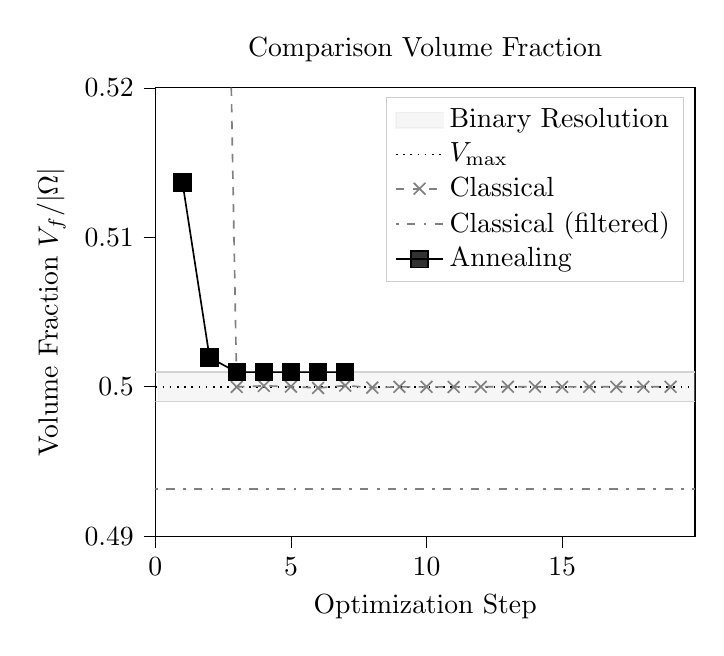
\begin{tikzpicture}

\definecolor{darkgray176}{RGB}{176,176,176}
\definecolor{gray}{RGB}{128,128,128}
\definecolor{lightgray}{RGB}{211,211,211}
\definecolor{lightgray204}{RGB}{204,204,204}

\begin{axis}[
legend cell align={left},
legend style={fill opacity=0.8, draw opacity=1, text opacity=1, draw=lightgray204},
tick align=outside,
tick pos=left,
title={Comparison Volume Fraction},
x grid style={darkgray176},
xlabel={Optimization Step},
xmin=0, xmax=19.9,
xtick style={color=black},
y grid style={darkgray176},
ylabel={Volume Fraction \(\displaystyle V_f/|\Omega|\)},
ymin=0.49, ymax=0.52,
ytick style={color=black}
]
\path [draw=lightgray, fill=lightgray, opacity=0.2]
(axis cs:0.1,0.5009765625)
--(axis cs:0.1,0.4990234375)
--(axis cs:0.3,0.4990234375)
--(axis cs:0.5,0.4990234375)
--(axis cs:0.7,0.4990234375)
--(axis cs:0.9,0.4990234375)
--(axis cs:1.1,0.4990234375)
--(axis cs:1.3,0.4990234375)
--(axis cs:1.5,0.4990234375)
--(axis cs:1.7,0.4990234375)
--(axis cs:1.9,0.4990234375)
--(axis cs:2.1,0.4990234375)
--(axis cs:2.3,0.4990234375)
--(axis cs:2.5,0.4990234375)
--(axis cs:2.7,0.4990234375)
--(axis cs:2.9,0.4990234375)
--(axis cs:3.1,0.4990234375)
--(axis cs:3.3,0.4990234375)
--(axis cs:3.5,0.4990234375)
--(axis cs:3.7,0.4990234375)
--(axis cs:3.9,0.4990234375)
--(axis cs:4.1,0.4990234375)
--(axis cs:4.3,0.4990234375)
--(axis cs:4.5,0.4990234375)
--(axis cs:4.7,0.4990234375)
--(axis cs:4.9,0.4990234375)
--(axis cs:5.1,0.4990234375)
--(axis cs:5.3,0.4990234375)
--(axis cs:5.5,0.4990234375)
--(axis cs:5.7,0.4990234375)
--(axis cs:5.9,0.4990234375)
--(axis cs:6.1,0.4990234375)
--(axis cs:6.3,0.4990234375)
--(axis cs:6.5,0.4990234375)
--(axis cs:6.7,0.4990234375)
--(axis cs:6.9,0.4990234375)
--(axis cs:7.1,0.4990234375)
--(axis cs:7.3,0.4990234375)
--(axis cs:7.5,0.4990234375)
--(axis cs:7.7,0.4990234375)
--(axis cs:7.9,0.4990234375)
--(axis cs:8.1,0.4990234375)
--(axis cs:8.3,0.4990234375)
--(axis cs:8.5,0.4990234375)
--(axis cs:8.7,0.4990234375)
--(axis cs:8.9,0.4990234375)
--(axis cs:9.1,0.4990234375)
--(axis cs:9.3,0.4990234375)
--(axis cs:9.5,0.4990234375)
--(axis cs:9.7,0.4990234375)
--(axis cs:9.9,0.4990234375)
--(axis cs:10.1,0.4990234375)
--(axis cs:10.3,0.4990234375)
--(axis cs:10.5,0.4990234375)
--(axis cs:10.7,0.4990234375)
--(axis cs:10.9,0.4990234375)
--(axis cs:11.1,0.4990234375)
--(axis cs:11.3,0.4990234375)
--(axis cs:11.5,0.4990234375)
--(axis cs:11.7,0.4990234375)
--(axis cs:11.9,0.4990234375)
--(axis cs:12.1,0.4990234375)
--(axis cs:12.3,0.4990234375)
--(axis cs:12.5,0.4990234375)
--(axis cs:12.7,0.4990234375)
--(axis cs:12.9,0.4990234375)
--(axis cs:13.1,0.4990234375)
--(axis cs:13.3,0.4990234375)
--(axis cs:13.5,0.4990234375)
--(axis cs:13.7,0.4990234375)
--(axis cs:13.9,0.4990234375)
--(axis cs:14.1,0.4990234375)
--(axis cs:14.3,0.4990234375)
--(axis cs:14.5,0.4990234375)
--(axis cs:14.7,0.4990234375)
--(axis cs:14.9,0.4990234375)
--(axis cs:15.1,0.4990234375)
--(axis cs:15.3,0.4990234375)
--(axis cs:15.5,0.4990234375)
--(axis cs:15.7,0.4990234375)
--(axis cs:15.9,0.4990234375)
--(axis cs:16.1,0.4990234375)
--(axis cs:16.3,0.4990234375)
--(axis cs:16.5,0.4990234375)
--(axis cs:16.7,0.4990234375)
--(axis cs:16.9,0.4990234375)
--(axis cs:17.1,0.4990234375)
--(axis cs:17.3,0.4990234375)
--(axis cs:17.5,0.4990234375)
--(axis cs:17.7,0.4990234375)
--(axis cs:17.9,0.4990234375)
--(axis cs:18.1,0.4990234375)
--(axis cs:18.3,0.4990234375)
--(axis cs:18.5,0.4990234375)
--(axis cs:18.7,0.4990234375)
--(axis cs:18.9,0.4990234375)
--(axis cs:19.1,0.4990234375)
--(axis cs:19.3,0.4990234375)
--(axis cs:19.5,0.4990234375)
--(axis cs:19.7,0.4990234375)
--(axis cs:19.9,0.4990234375)
--(axis cs:19.9,0.5009765625)
--(axis cs:19.9,0.5009765625)
--(axis cs:19.7,0.5009765625)
--(axis cs:19.5,0.5009765625)
--(axis cs:19.3,0.5009765625)
--(axis cs:19.1,0.5009765625)
--(axis cs:18.9,0.5009765625)
--(axis cs:18.7,0.5009765625)
--(axis cs:18.5,0.5009765625)
--(axis cs:18.3,0.5009765625)
--(axis cs:18.1,0.5009765625)
--(axis cs:17.9,0.5009765625)
--(axis cs:17.7,0.5009765625)
--(axis cs:17.5,0.5009765625)
--(axis cs:17.3,0.5009765625)
--(axis cs:17.1,0.5009765625)
--(axis cs:16.9,0.5009765625)
--(axis cs:16.7,0.5009765625)
--(axis cs:16.5,0.5009765625)
--(axis cs:16.3,0.5009765625)
--(axis cs:16.1,0.5009765625)
--(axis cs:15.9,0.5009765625)
--(axis cs:15.7,0.5009765625)
--(axis cs:15.5,0.5009765625)
--(axis cs:15.3,0.5009765625)
--(axis cs:15.1,0.5009765625)
--(axis cs:14.9,0.5009765625)
--(axis cs:14.7,0.5009765625)
--(axis cs:14.5,0.5009765625)
--(axis cs:14.3,0.5009765625)
--(axis cs:14.1,0.5009765625)
--(axis cs:13.9,0.5009765625)
--(axis cs:13.7,0.5009765625)
--(axis cs:13.5,0.5009765625)
--(axis cs:13.3,0.5009765625)
--(axis cs:13.1,0.5009765625)
--(axis cs:12.9,0.5009765625)
--(axis cs:12.7,0.5009765625)
--(axis cs:12.5,0.5009765625)
--(axis cs:12.3,0.5009765625)
--(axis cs:12.1,0.5009765625)
--(axis cs:11.9,0.5009765625)
--(axis cs:11.7,0.5009765625)
--(axis cs:11.5,0.5009765625)
--(axis cs:11.3,0.5009765625)
--(axis cs:11.1,0.5009765625)
--(axis cs:10.9,0.5009765625)
--(axis cs:10.7,0.5009765625)
--(axis cs:10.5,0.5009765625)
--(axis cs:10.3,0.5009765625)
--(axis cs:10.1,0.5009765625)
--(axis cs:9.9,0.5009765625)
--(axis cs:9.7,0.5009765625)
--(axis cs:9.5,0.5009765625)
--(axis cs:9.3,0.5009765625)
--(axis cs:9.1,0.5009765625)
--(axis cs:8.9,0.5009765625)
--(axis cs:8.7,0.5009765625)
--(axis cs:8.5,0.5009765625)
--(axis cs:8.3,0.5009765625)
--(axis cs:8.1,0.5009765625)
--(axis cs:7.9,0.5009765625)
--(axis cs:7.7,0.5009765625)
--(axis cs:7.5,0.5009765625)
--(axis cs:7.3,0.5009765625)
--(axis cs:7.1,0.5009765625)
--(axis cs:6.9,0.5009765625)
--(axis cs:6.7,0.5009765625)
--(axis cs:6.5,0.5009765625)
--(axis cs:6.3,0.5009765625)
--(axis cs:6.1,0.5009765625)
--(axis cs:5.9,0.5009765625)
--(axis cs:5.7,0.5009765625)
--(axis cs:5.5,0.5009765625)
--(axis cs:5.3,0.5009765625)
--(axis cs:5.1,0.5009765625)
--(axis cs:4.9,0.5009765625)
--(axis cs:4.7,0.5009765625)
--(axis cs:4.5,0.5009765625)
--(axis cs:4.3,0.5009765625)
--(axis cs:4.1,0.5009765625)
--(axis cs:3.9,0.5009765625)
--(axis cs:3.7,0.5009765625)
--(axis cs:3.5,0.5009765625)
--(axis cs:3.3,0.5009765625)
--(axis cs:3.1,0.5009765625)
--(axis cs:2.9,0.5009765625)
--(axis cs:2.7,0.5009765625)
--(axis cs:2.5,0.5009765625)
--(axis cs:2.3,0.5009765625)
--(axis cs:2.1,0.5009765625)
--(axis cs:1.9,0.5009765625)
--(axis cs:1.7,0.5009765625)
--(axis cs:1.5,0.5009765625)
--(axis cs:1.3,0.5009765625)
--(axis cs:1.1,0.5009765625)
--(axis cs:0.9,0.5009765625)
--(axis cs:0.7,0.5009765625)
--(axis cs:0.5,0.5009765625)
--(axis cs:0.3,0.5009765625)
--(axis cs:0.1,0.5009765625)
--cycle;
\addlegendimage{area legend, draw=lightgray, fill=lightgray, opacity=0.2}
\addlegendentry{Binary Resolution}

\addplot [semithick, black, dotted]
table {%
0 0.5
19.9 0.5
};
\addlegendentry{$V_{\mathrm{max}}$}
\addplot [semithick, lightgray, forget plot]
table {%
0 0.5009765625
19.9 0.5009765625
};
\addplot [semithick, lightgray, forget plot]
table {%
0 0.4990234375
19.9 0.4990234375
};
\addplot [semithick, gray, dashed, mark=x, mark size=3, mark options={solid}]
table {%
1 0.8
2 0.6
3 0.499989219033465
4 0.500060363597868
5 0.500011010448369
6 0.499917531192211
7 0.500077014869896
8 0.499945280509116
9 0.49999481202698
10 0.499994950315845
11 0.499988577673993
12 0.499996091633121
13 0.500002956909401
14 0.500000596249279
15 0.499990044013989
16 0.499998153540262
17 0.499997710184589
18 0.499999898925017
19 0.499997821479091
};
\addlegendentry{Classical}
\addplot [semithick, gray, dash pattern=on 1pt off 3pt on 3pt off 3pt]
table {%
0 0.4931640625
19.9 0.4931640625
};
\addlegendentry{Classical (filtered)}
\addplot [semithick, black, mark=square*, mark size=3, mark options={solid}]
table {%
1 0.513671875
2 0.501953125
3 0.5009765625
4 0.5009765625
5 0.5009765625
6 0.5009765625
7 0.5009765625
};
\addlegendentry{Annealing}
\end{axis}

\end{tikzpicture}
